\section{Experiments}
\subsection{Relative Machine Precision}
ab4.py gives us the following table (see figure \ref{fig:cmd_epsilon}) for the relative machine precision of np.float16, np.float32 and np.float64.
\begin{figure}[ht]
    \centering
        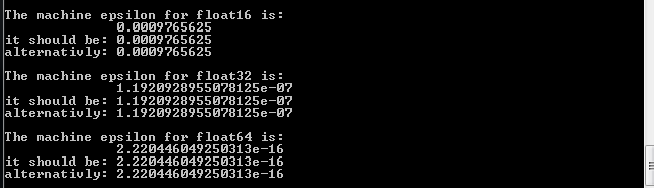
\includegraphics[width=0.9\textwidth]{graphics/cmd_epsilon}
    \caption{command line output of ab4.py regarding different floating types}\label{fig:cmd_epsilon}
\end{figure}\\
np.float16, np.float32 and np.float 64 have 10 bit, 23 bit, 52 bit mantissa respectively \cite{bib:numpy}. According to the definition of relative machine precision, we have
\begin{align*}
    \tau_{16} &= 2^{-10} = 0.0009765625 \\
    \tau_{32} &= 2^{-23} = 1.1920928955078125 \times 10^{-7} \\
    \tau_{64} &= 2^{-52} \approx 2.220446049250313 \times 10^{-16}
\end{align*}
verifying our theory. \\
An interesting observation is that with each bit, the floating number becomes more precise, however this precision growth is not linear since \(\tau = \frac{1}{2^t}\). Considering that each new bit is less effective than the last in terms of improving the precision, there should be a practical limit for the hard ware.
\subsection{Rounding Error and Absorbtion}
We will consider the plots of the absolute and the relative errors for values
\begin{align*}
    x_1 &= 7733 & \text{ see figure \ref{fig:7733}}\\
    x_2 &= 100,000,000,011 & \text{ see figure \ref{fig:1011}}\\
    x_3 &= 2,222,222,222,222,222,222,222 & \text{(22 times 2; see figure \ref{fig:2times22})} \text{.}
\end{align*}
\begin{figure}[p]
    \centering
        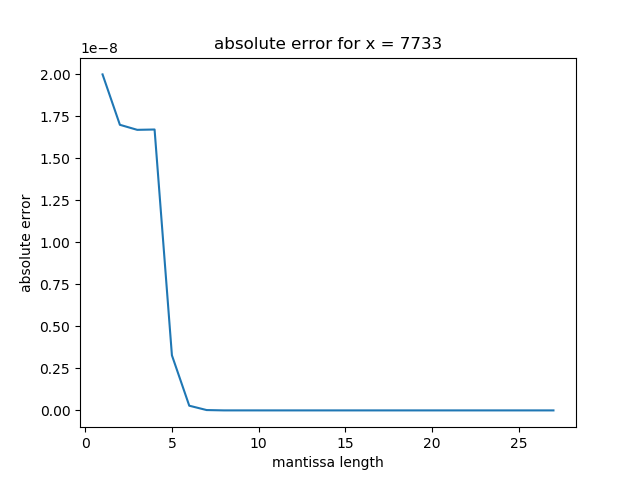
\includegraphics[width=0.5\textwidth]{graphics/abs7733}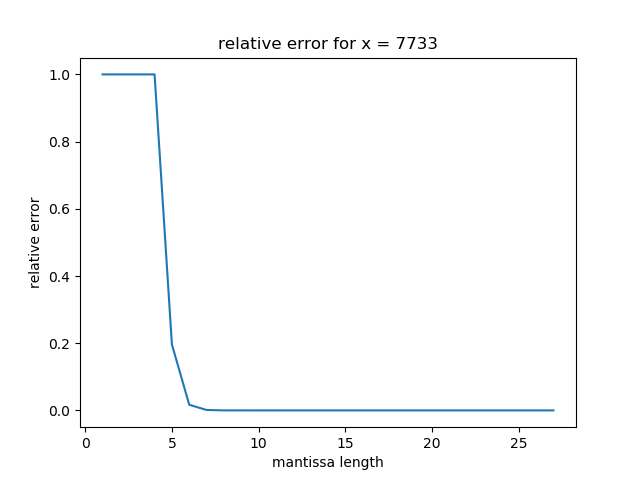
\includegraphics[width=0.5\textwidth]{graphics/rel7733}
    \caption{absolute and relative error plot for x = 7733}\label{fig:7733}
    \centering
        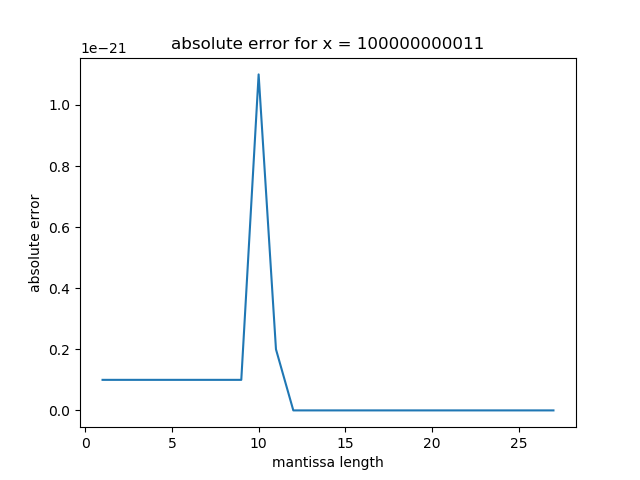
\includegraphics[width=0.5\textwidth]{graphics/abs100000000011}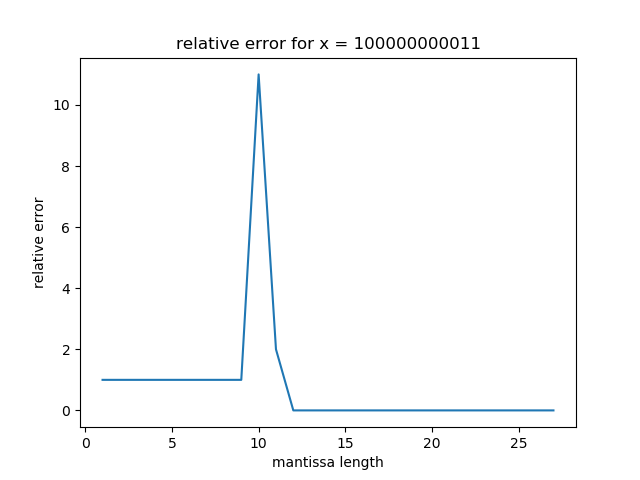
\includegraphics[width=0.5\textwidth]{graphics/rel100000000011}
    \caption{absolute and relative error plot for x = 100000000011}\label{fig:1011}
    \centering
        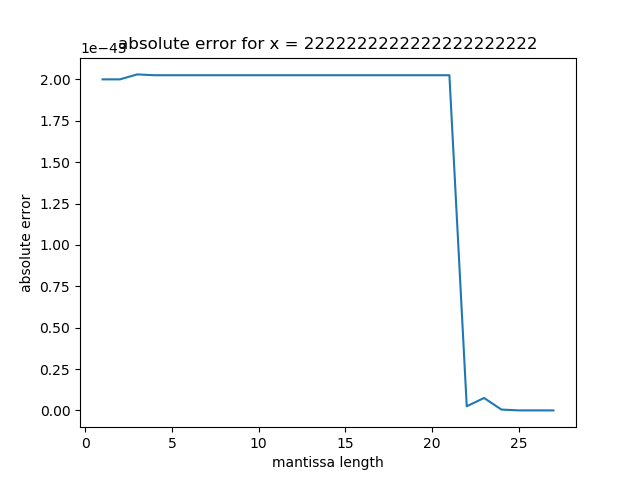
\includegraphics[width=0.5\textwidth]{graphics/abs2times22}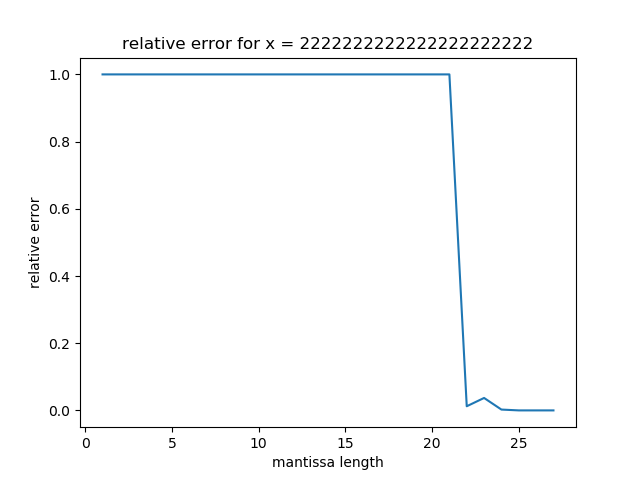
\includegraphics[width=0.5\textwidth]{graphics/rel2times22}
    \caption{absolute and relative error plot for x = 2,222,222,222,222,222,222,222}\label{fig:2times22}
\end{figure}
As one can see on every plot, the plot of the absolute and relative error becomes 0 (or at least very close to) if the mantissa length is longer than number of digit of x. This means that if one wants to compute something in the floating algorithm, they should choose the mantissa to be as long as (preferably longer) than the maximum number of digits in their calculations.